%!TEX root = ../08-Interference.tex
\chapter{Newton's Rings}

The curvature radius of a biconvex lens and the refractive index of water are determined by analyzing the lense's Newton's rings interference pattern.

\addsec{Setup}

Newton's rings is an interference phenomena that occurs when a transparent spherical object is placed on a flat reflective surface and is illuminated from the top with monochromatic, coherent light.
A series of concentric rings can be observed.

A portion of the incident light is reflected when exiting the lens, the light \todo{bla bla bla}
The two beams have a path difference of $2 d$, additionally a phase inversion occurs at the substrate, where the light enters a more optically dense medium.

The geometry of the spherical lens gives $d = \frac{r^2}{R}$, where $R$ is the curvature radius of the lens and $r$ is the horizontal radius from the contact point of the lens and substrate.

Substituting this into the condition for destructive interference $2 d \cdot n = k \lambda$ gives
\begin{equation}\label{eq:newton}
	\frac{r_k^2}{R} = \frac{k \lambda}{n} \quad \Leftrightarrow \quad \frac{r_k^2}{k} = \frac{R \lambda}{n},
\end{equation}
where $n$ is the index of refraction of the medium between the lens and substrate.
The ratio $\frac{r_k^2}{k}$ is constant, it can be determined using linear regression.

The reflections that occur at the top of the lens and the bottom of the substrate do not produce interference patterns, as the path differences are much larger than the coherence length of tyical LEDs.

A microscope slide is used as the substrate.
The lens and substrate are placed in a microscope with a XY-stage and a vernier scale on both axes.
The rings are centered around the crosshair.
A crosshair is used to find the edges of the rings along one axis, the rings' radii are read on the vernier scale.

To shorten the calculations, the refractive index of air is assumed to be exactly \num{1}.

\begin{figure}[tbp]
	\centering
	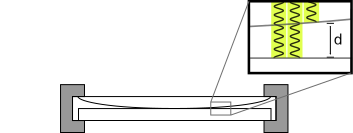
\includegraphics[width=.6\textwidth]{img/newtons-rings.pdf}
	\caption{Newton's Rings}
	\caption*{based on \url{https://en.wikipedia.org/wiki/Newton\%27s_rings\#/media/File:Newton\%27s_rings_02.svg}}
\end{figure}

\section{Measuring the Radius of Curvature}\label{sec:radius}

\begin{figure}[tbp]
	\centering
	\begin{subfigure}{.49\textwidth}
		\centering
		\includegraphics[width=1.1\textwidth]{data/plots/1-1-blue.pdf}
		\caption{Blue LED (\SI{465}{\nm})}
		\caption*{$\frac{r_k^2}{k} = \SI{0.154}{\mm\squared}$}
	\end{subfigure}
	\begin{subfigure}{.49\textwidth}
		\centering
		\includegraphics[width=1.1\textwidth]{data/plots/1-1-yellow.pdf}
		\caption{Yellow LED (\SI{590}{\nm})}
		\caption*{$\frac{r_k^2}{k} = \SI{0.173}{\mm\squared}$}
	\end{subfigure}
	\caption{Newton's Rings in Air}
\end{figure}

Radii for rings of all discernible orders are measured with yellow and blue light.
Solving \autoref{eq:newton} for $R$ and substituting the wavelengths and slopes of the lienar fits, this yields $R_\text{blue} = \SI{0.33}{\meter}$ and $R_\text{yellow} = \SI{0.29}{\meter}$.

\section{Index of Refraction of Water}

The experiment is repeated with yellow light and water between the substrate and lens.
The slope of the linear fit is $\frac{r_k^2}{k} = \SI{0.146}{\mm\squared}$ giving an uncorrected radius of $R_\text{water} = \SI{0.25}{\meter}$.
To increase accuracy, both measurements from \autoref{sec:radius} are averaged to form the reference value.
The radii of curvature $R$ are used instead of the slopes, as they are independent of the wavelength, the average radius in air is $\langle R_\text{air} \rangle = \SI{0.31}{\meter}$.

The index of refraction of water is calculated as
\begin{equation*}
	n_\text{water} = \frac{\langle R_\text{air} \rangle}{R_\text{water}} = \num{1.26},
\end{equation*}
which deviates from the literature value of $n_\text{lit,water} = \num{1.33}$ by \SI{5}{\percent}.

\section{Focal Length of the Lens}
